%-------------------------------------------- 6.1  
\subsection{\hll{Numbering in few columns}}
\begin{table}[h!]
\begin{tabular}{c | c}
\begin{minipage}[m]{0.4\textwidth}
\enum{
\begin{multicols}{2}%change to have more columns 
\begin{enumerate}
\item c
\item g
\item d
\item f
\end{enumerate}
\end{multicols}}{6.1}
\end{minipage}
&
\begin{minipage}[m]{0.55\textwidth}
\renewcommand\textminus{\mbox{-}}%<<<<<<<<<<<
\begin{lstlisting}[numberstyle=\zebra{blue!15}{orange!15},numbers=left,basicstyle=\ttfamily\scriptsize]{tex}
\documentclass{article}
\usepackage{multicol} 

\begin{document}
\begin{multicols}{2}%change to have more columns 
\begin{enumerate}
\item c
\item g
\item d
\item f
\end{enumerate}
\end{multicols}
\end{document}
\end{lstlisting}
\end{minipage}
\end{tabular}
\end{table}

%-------------------------------------------- 6.2
\subsection{\hll{Enumeration environment with position number in the format (i, j)}}
\begin{table}[h!]
\begin{tabular}{c | c}
\begin{minipage}[m]{0.4\textwidth}
\enum{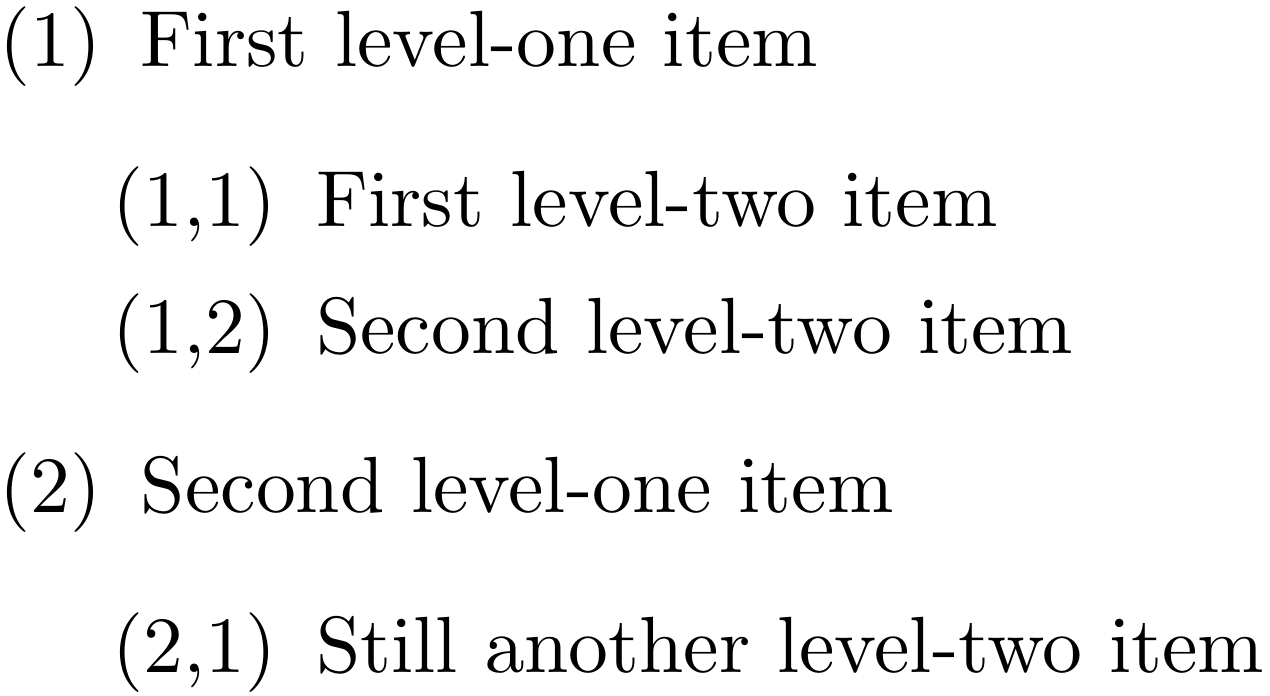
\includegraphics[width=0.9\linewidth]{6.2.png}}{6.2}
\end{minipage}
&
\begin{minipage}[m]{0.55\textwidth}
\renewcommand\textminus{\mbox{-}}%<<<<<<<<<<<
\begin{lstlisting}[numberstyle=\zebra{blue!15}{orange!15},numbers=left,basicstyle=\ttfamily\scriptsize] 
\documentclass{article}
\renewcommand{\theenumi}{(\arabic{enumi})}
\renewcommand{\theenumii}{(\arabic{enumi},\arabic{enumii})}
\renewcommand{\labelenumi}{\theenumi}
\renewcommand{\labelenumii}{\theenumii}
\makeatletter \renewcommand{\p@enumii}{} \makeatother

\begin{document}
\begin{enumerate}
\item First level-one item 
  \begin{enumerate}
  \item First level-two item 
  \item Second level-two item
  \end{enumerate}
\item Second level-one item 
  \begin{enumerate}
  \item Still another level-two item 
  \end{enumerate}
\end{enumerate}
\end{document} 
\end{lstlisting}
\end{minipage}
\end{tabular}
\end{table}

\newpage
%-------------------------------------------- 6.3  
\subsection{\hll{Colored enumeration}}
\begin{table}[h!]
\begin{tabular}{c | c}
\begin{minipage}[m]{0.4\textwidth}
\enum{ \renewcommand{\labelenumi}{\SebastianoItem{\arabic{enumi}}}
  \begin{enumerate}
   \item \href{https://tex.stackexchange.com/questions/430542/a-fancy-and-beautiful-type-of-enumerate}{item}
    \item \item \href{https://tex.stackexchange.com/questions/430542/a-fancy-and-beautiful-type-of-enumerate}{item}
    \item \item \href{https://tex.stackexchange.com/questions/430542/a-fancy-and-beautiful-type-of-enumerate}{special item} \SebastianoHighlight
    \item \item \href{https://tex.stackexchange.com/questions/430542/a-fancy-and-beautiful-type-of-enumerate}{item}
  \end{enumerate}}{6.3}
\end{minipage}
&
\begin{minipage}[m]{0.55\textwidth}
\renewcommand\textminus{\mbox{-}}%<<<<<<<<<<<
\begin{lstlisting}[numberstyle=\zebra{blue!15}{orange!15},numbers=left,basicstyle=\ttfamily\scriptsize] 
\documentclass{article}
\usepackage{tikz}
\definecolor{amethyst}{rgb}{0.6, 0.4, 0.8}
\definecolor{applegreen}{rgb}{0.55, 0.71, 0.0}
\definecolor{arylideyellow}{rgb}{0.91, 0.84, 0.42}
\definecolor{asparagus}{rgb}{0.53, 0.66, 0.42}
\definecolor{atomictangerine}{rgb}{1.0, 0.6, 0.4}
\definecolor{bananayellow}{rgb}{1.0, 0.88, 0.21}
\definecolor{brightgreen}{rgb}{0.4, 1.0, 0.0}
\definecolor{cambridgeblue}{rgb}{0.64, 0.76, 0.68}
\definecolor{capri}{rgb}{0.0, 0.75, 1.0}
\definecolor{carnationpink}{rgb}{1.0, 0.65, 0.79}
\newcommand{\ClaudioList}{red,applegreen,amethyst,carnationpink,blue!50!cyan,arylideyellow,asparagus,atomictangerine,bananayellow,brightgreen,cambridgeblue,capri}
\newcommand{\SebastianoItem}[1]{\foreach \X[count=\Y] in \ClaudioList
{\ifnum\Y=#1\relax
\xdef\SebastianoColor{\X}
\fi}
\tikz[baseline=(SebastianoItem.base),remember
picture]{%
\node[fill=\SebastianoColor,inner sep=4pt,font=\sffamily,fill opacity=0.5] (SebastianoItem){#1)};}}
\newcommand{\SebastianoHighlight}{\tikz[overlay,remember picture]{%
\fill[\SebastianoColor,fill opacity=0.5] ([yshift=4pt,xshift=-\pgflinewidth]SebastianoItem.east) -- ++(4pt,-4pt)
-- ++(-4pt,-4pt) -- cycle;}}

\begin{document}
\renewcommand{\labelenumi}{\SebastianoItem{\arabic{enumi}}}
  \begin{enumerate}
    \item item
    \item special item \SebastianoHighlight
    \item item
  \end{enumerate}
\end{document}
\end{lstlisting}
\end{minipage}
\end{tabular}
\end{table}
%-------------------------------------------- 6.4  
\subsection{\hll{Leveled arabic enumeration}}
\begin{table}[h!]
\begin{tabular}{c | c}
\begin{minipage}[m]{0.4\textwidth}
\enum{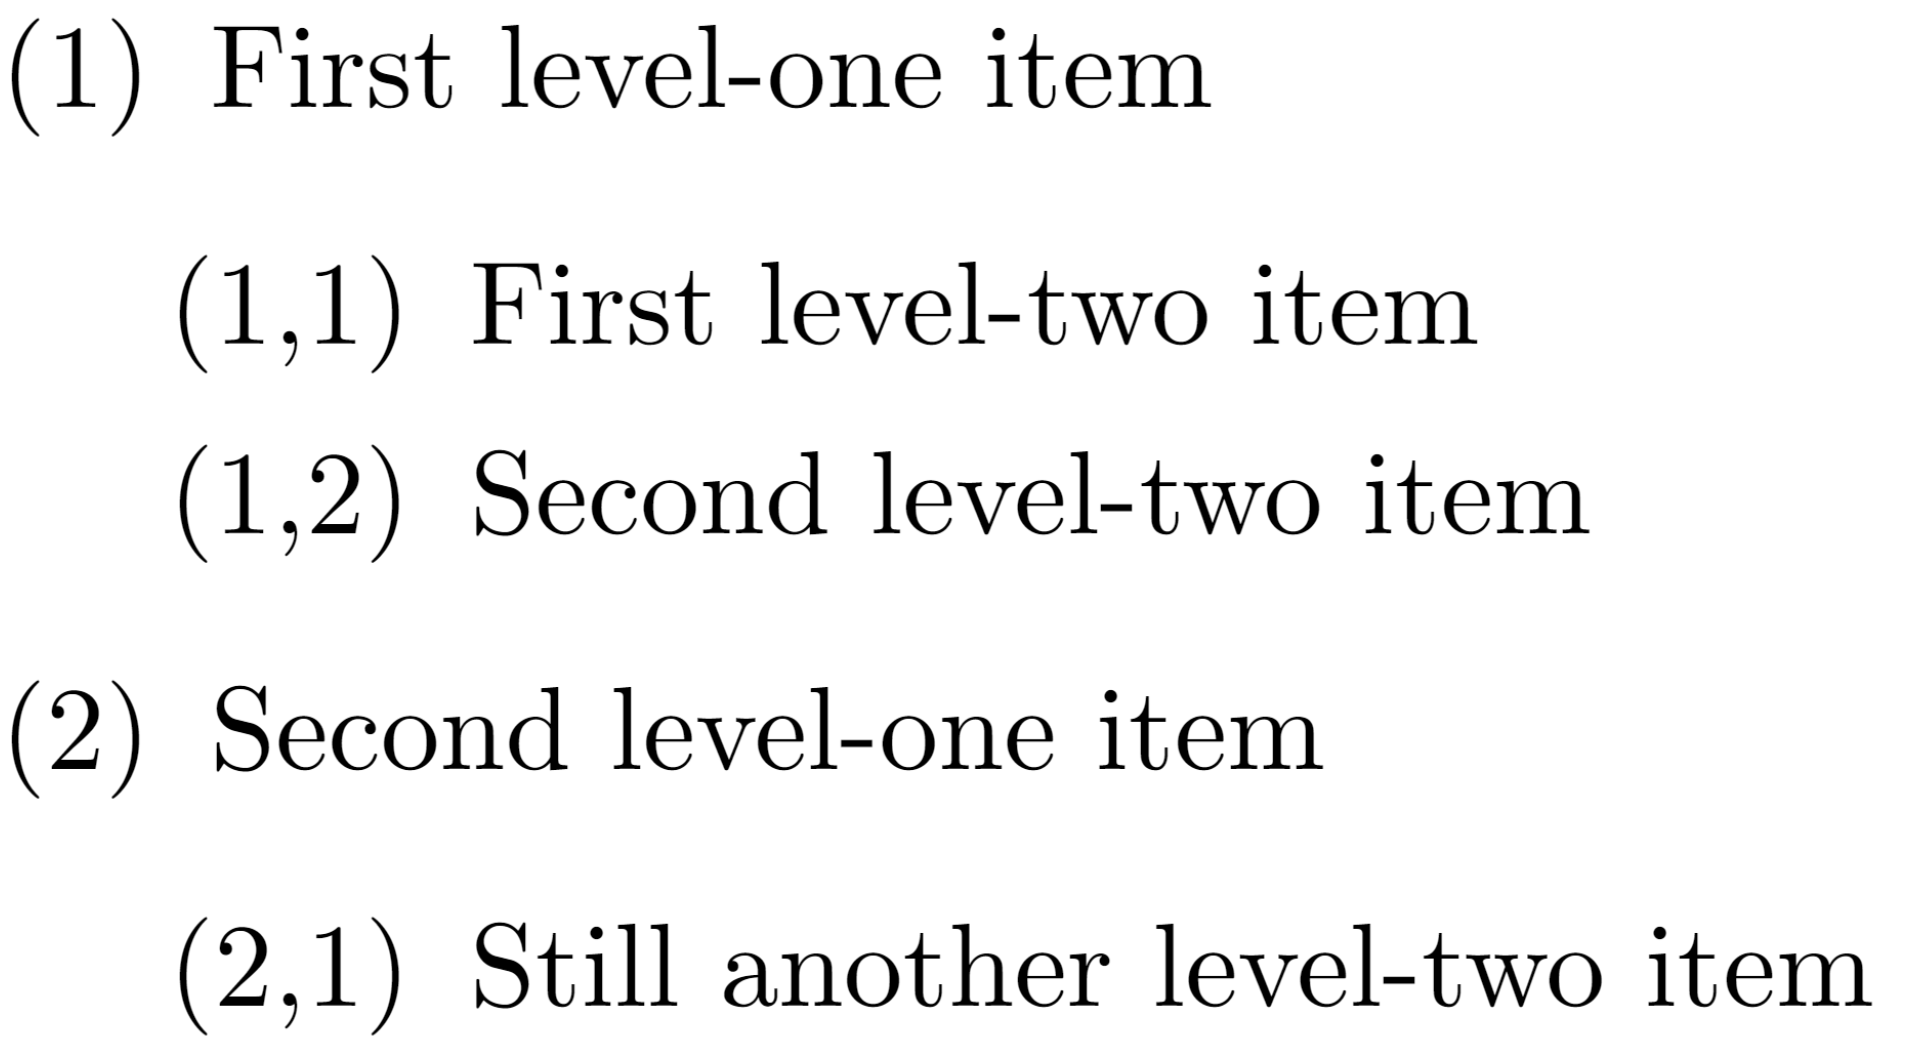
\includegraphics[width=0.9\linewidth]{6.4.png}}{6.4}
\end{minipage}
&
\begin{minipage}[m]{0.55\textwidth}
\renewcommand\textminus{\mbox{-}}%<<<<<<<<<<<
\begin{lstlisting}[numberstyle=\zebra{blue!15}{orange!15},numbers=left,basicstyle=\ttfamily\scriptsize] 
\documentclass{article}
\renewcommand{\theenumi}{(\arabic{enumi})}
\renewcommand{\theenumii}{(\arabic{enumi},\arabic{enumii})}
\renewcommand{\labelenumi}{\theenumi}
\renewcommand{\labelenumii}{\theenumii}
\makeatletter
\renewcommand{\p@enumii}{}
\makeatother
\begin{document}
\begin{enumerate}
\item First level-one item 
  \begin{enumerate}
  \item First level-two item 
  \item Second level-two item
  \end{enumerate}
\item Second level-one item 
  \begin{enumerate}
  \item Still another level-two item 
  \end{enumerate}
\end{enumerate}
\end{document} 
\end{lstlisting}
\end{minipage}
\end{tabular}
\end{table}
%-------------------------------------------- 6.5 
\subsection{\hll{Change footnote symbol}}
\begin{table}[h!]
\begin{tabular}{c | c}
\begin{minipage}[m]{0.4\textwidth}
\enum{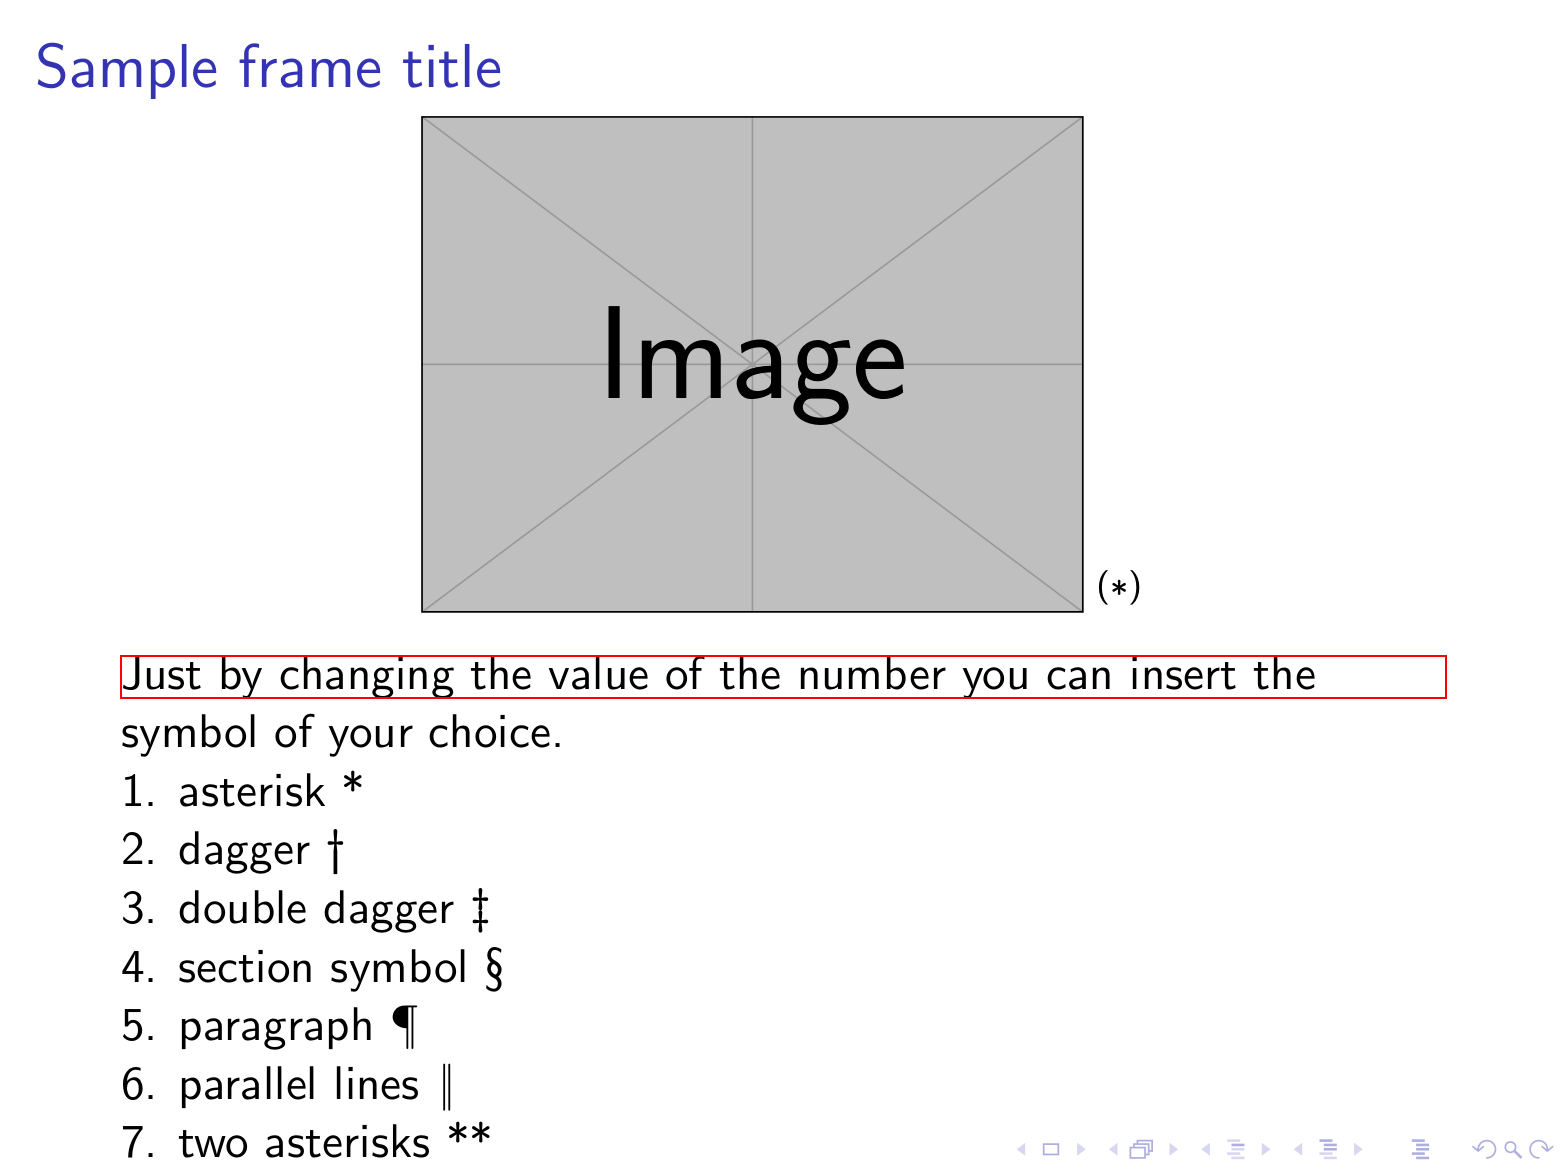
\includegraphics[width=0.9\linewidth]{6.5.png}}{6.5}
\end{minipage}
&
\begin{minipage}[m]{0.55\textwidth}
\renewcommand\textminus{\mbox{-}}%<<<<<<<<<<<
\begin{lstlisting}[numberstyle=\zebra{blue!15}{orange!15},numbers=left,basicstyle=\ttfamily\scriptsize] 
\documentclass{beamer}
\renewcommand{\thefootnote}{ (\fnsymbol{footnote})}

\begin{document}
\begin{frame}
\frametitle{Sample frame title}
\begin{figure}
\includegraphics[width=0.5\linewidth]{example-image}\footnote[1]{image description}
\end{figure}
\end{frame}
\end{document}
\end{lstlisting}
\end{minipage}
\end{tabular}
\end{table} 
%-------------------------------------------- 6.6  
\subsection{\hll{Bullets Style}}
\begin{table}[h!]
\begin{tabular}{c | c}
\begin{minipage}[m]{0.4\textwidth}
\enum{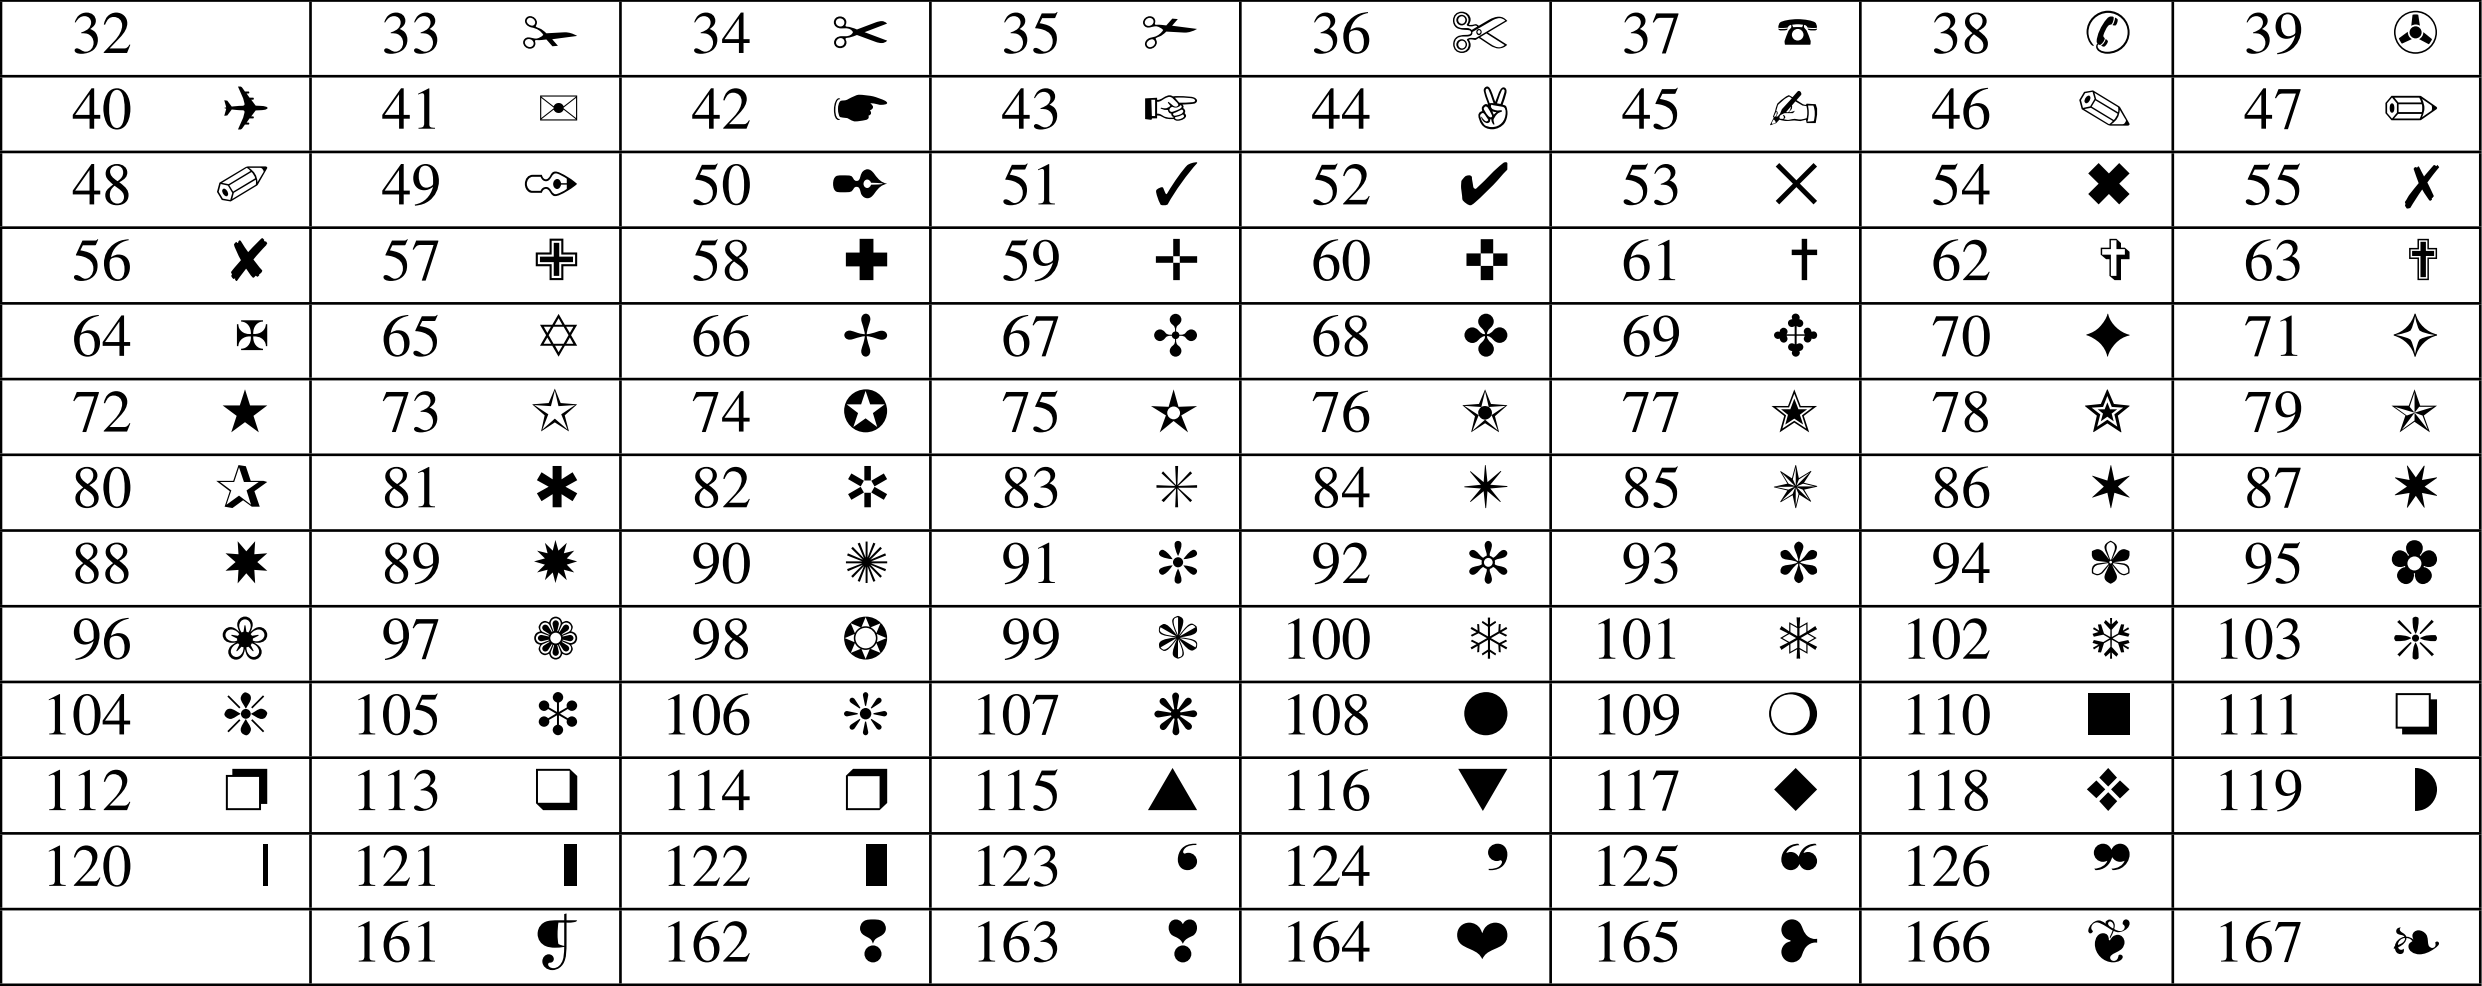
\includegraphics[width=\linewidth]{6.6.1.png}
\begin{itemize}
    \item[\ding{51}] Code 51
    \item[\ding{56}] Code 56
    \item[\ding{43}] Code 43
    \item[\ding{118}] Code 118
    \item[\ding{170}] Code 170
\end{itemize}
\par
\ding{46} \ding{70} \ding{57}  \ding{98} \ding{96}
 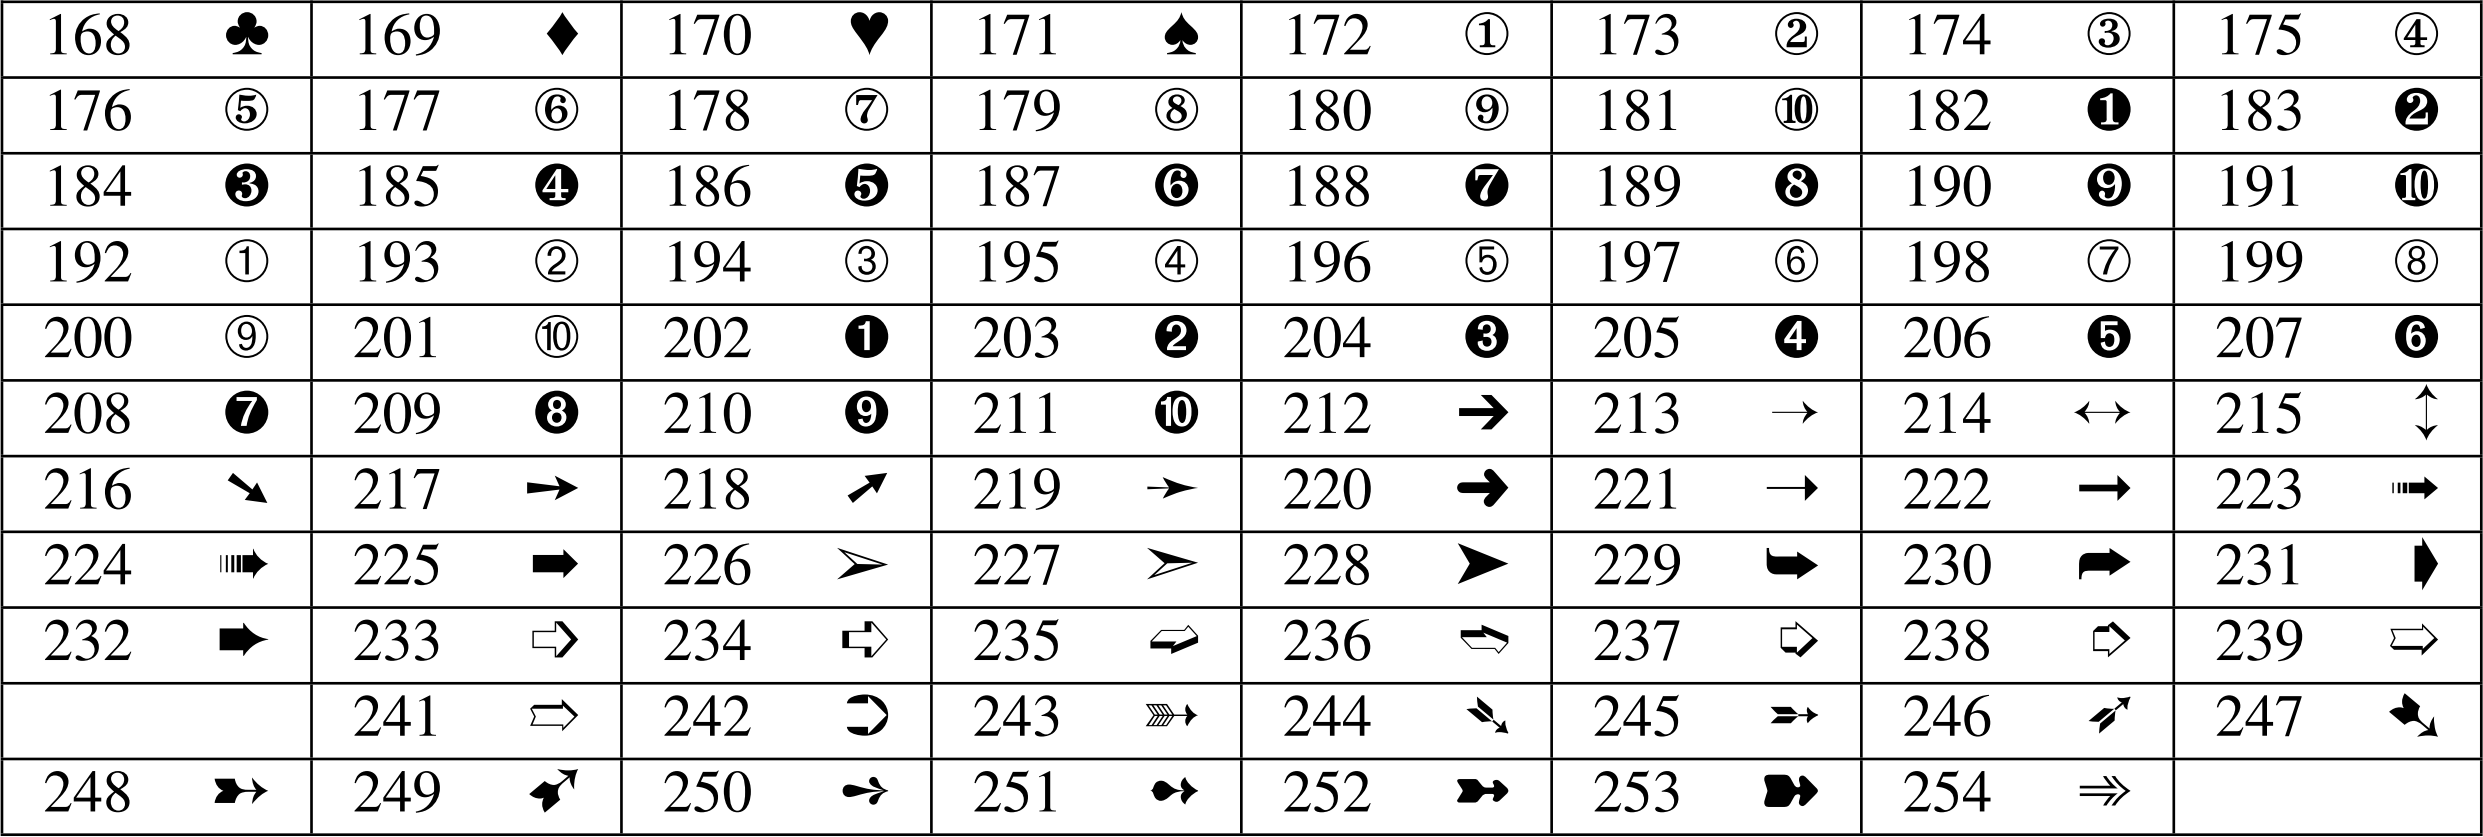
\includegraphics[width=\linewidth]{6.6.2.png}}{2.4}
\end{minipage}
&
\begin{minipage}[m]{0.55\textwidth}
\renewcommand\textminus{\mbox{-}}%<<<<<<<<<<<
\begin{lstlisting}[numberstyle=\zebra{red!15}{black!10},numbers=left,basicstyle=\ttfamily\footnotesize] 
\documentclass{article}
\usepackage{pifont}

\begin{document}
\begin{itemize}
    \item[\ding{51}] Code 51
    \item[\ding{56}] Code 56
    \item[\ding{43}] Code 43
    \item[\ding{118}] Code 118
    \item[\ding{170}] Code 170
\end{itemize}
\par
\ding{46} \ding{70} \ding{57}  \ding{98} \ding{96}
\end{document}
\end{lstlisting}
\end{minipage}
\end{tabular}
\end{table}
%-------------------------------------------- 6.7  
  
